\documentclass[a4paper,12pt]{article}
\usepackage{amsmath, amssymb, siunitx, graphicx}
\usepackage{hyperref}
\usepackage{float}
\usepackage{tikz}
\usepackage{pgfplots}
\pgfplotsset{compat=1.18}
\title{Transient Response Analysis of an LC Circuit}
\author{EE24BTECH11048-NITHIN.K \\ EE24BTECH11021-ESHAN RAY}
\date{\today}

\begin{document}

\maketitle

\section{Objective}
To study and analyze the transient response of an LC circuit, determine the natural frequency (\(\Omega_n\)), and calculate the damping ratio (\(\xi\)) using theoretical and experimental methods.

\section{Equipment Required}
\begin{itemize}
    \item \SI{472}{p\farad} capacitor
    \item \SI{2.2}{\milli\henry} inductor
    \item Small-value resistor (if needed)
    \item DC power supply (\SI{5}{V})
    \item Oscilloscope
    \item Connecting wires
\end{itemize}

\section{Theory}
An LC circuit consists of an inductor (\(L\)) and a capacitor (\(C\)) connected in parallel. When a charged capacitor is connected to an inductor, energy oscillates between the capacitor's electric field and the inductor's magnetic field. The ideal LC circuit follows the second-order differential equation:
\begin{equation*}
    L \frac{d^2q}{dt^2} + \frac{q}{C} = 0
\end{equation*}
where \(q\) is the charge on the capacitor. The natural frequency of oscillation is given by:
\begin{equation*}
    \Omega_n = \frac{1}{\sqrt{LC}}
\end{equation*}

However, in real components, the inductor and capacitor have inherent resistance (R), forming an RLC circuit. The presence of resistance introduces damping, and the damping ratio (\(\xi\)) is given by:
\begin{equation*}
    \xi = \frac{R}{2} \sqrt{\frac{C}{L}}
\end{equation*}

The damped frequency (\(\Omega_d\)) is related to the natural frequency as:
\begin{equation*}
    \Omega_d = \Omega_n \sqrt{1 - \xi^2}
\end{equation*}

\section{Procedure}
\subsection{Precharging the Capacitor}
\begin{enumerate}
    \item Connect the \SI{100}{\micro\farad} capacitor to a \SI{5}{V} DC power supply.
    \item Once fully charged, disconnect it carefully without discharging.
\end{enumerate}

\subsection{Constructing the LC Circuit}
\begin{enumerate}
    \item Connect the charged capacitor in parallel with the \SI{2.2}{\milli\henry} inductor as shown in the figure below.
    \item Ensure minimal resistance in wiring.
\end{enumerate}
\begin{figure}[H]
    \centering
    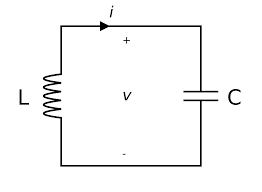
\includegraphics[width=0.7\textwidth]{figs/diagram.png}
    \caption{Diagram for LC circuit}
\end{figure}
\begin{figure}[H]
    \centering
    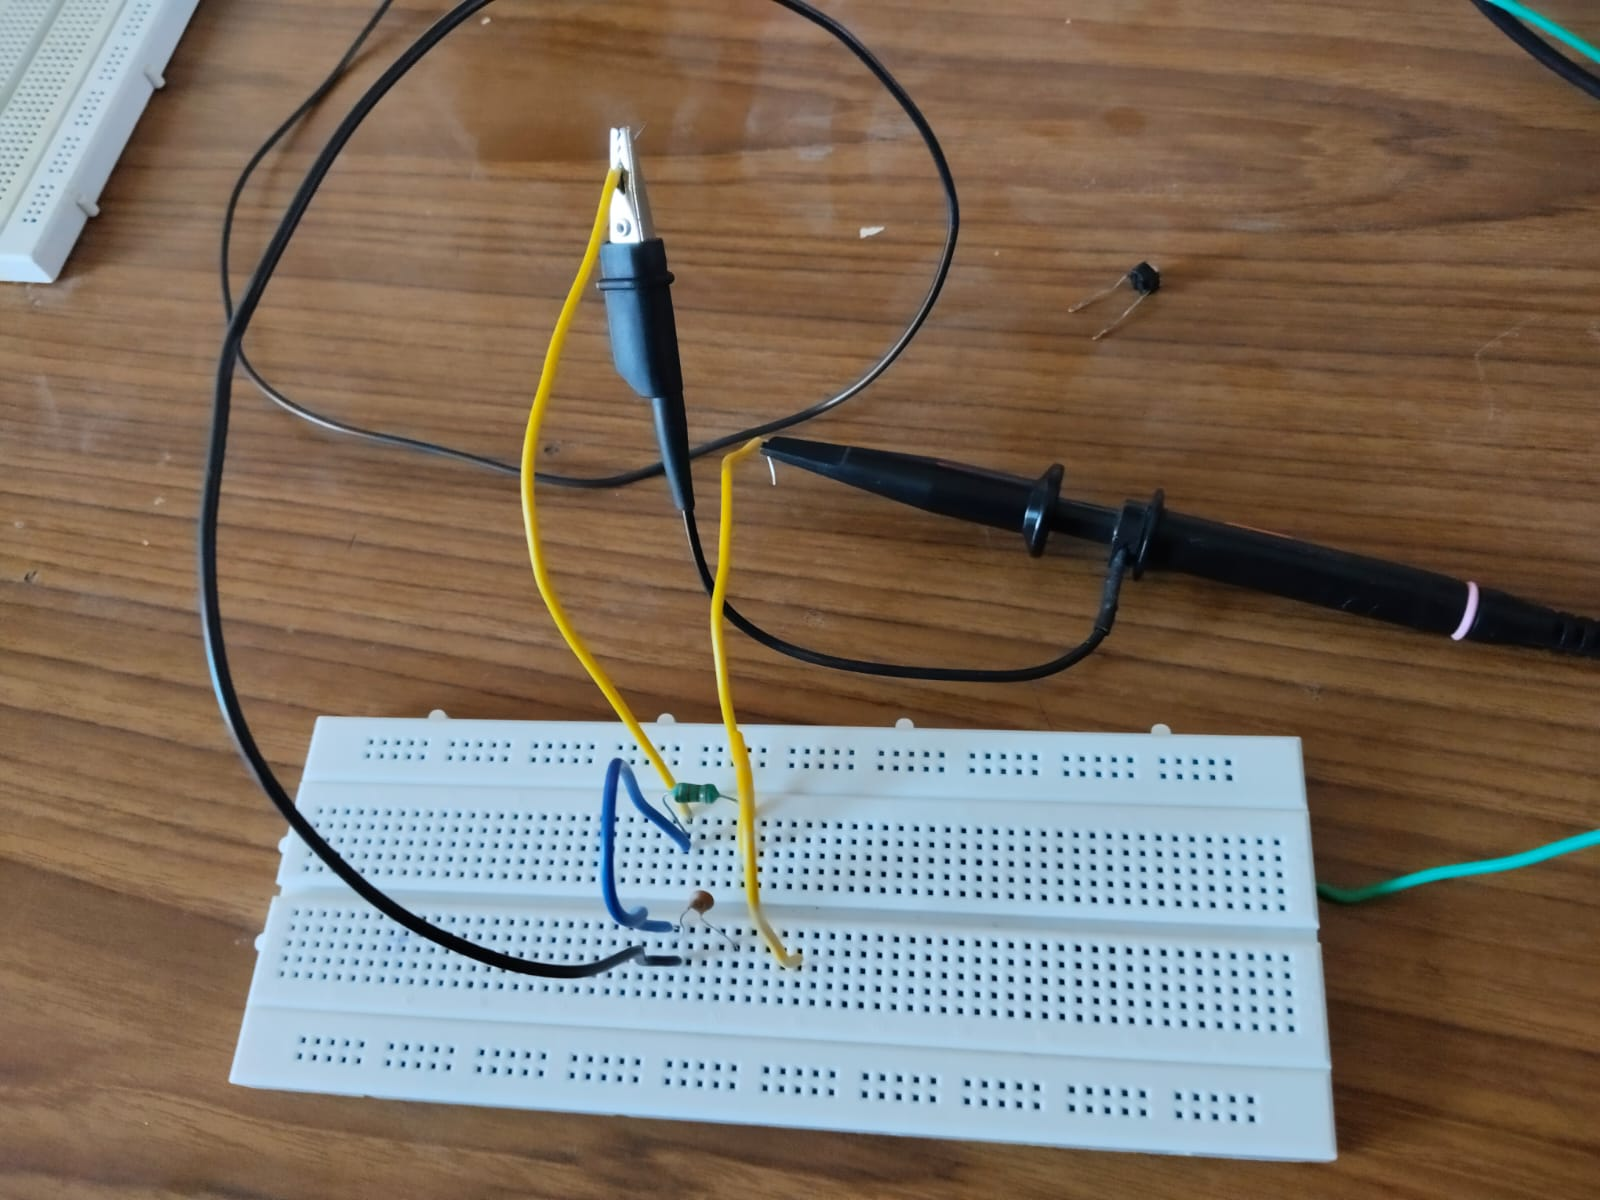
\includegraphics[width=0.7\textwidth]{figs/circuit.jpeg}
    \caption{LC Circuit}
\end{figure}
\subsection{Capturing the Transient Response}
\begin{enumerate}
    \item Use an oscilloscope to monitor the voltage across the inductor.
    \item Observe the natural oscillations and measure the oscillation period.
\end{enumerate}

\subsection{Theoretical Calculations}
\begin{enumerate}
    \item Compute \(\Omega_n\) using the given values of \(L\) and \(C\).
    \item Calculate the damping ratio \(\xi\) using measured resistance.
\end{enumerate}
\begin{figure}[H]
    \centering
    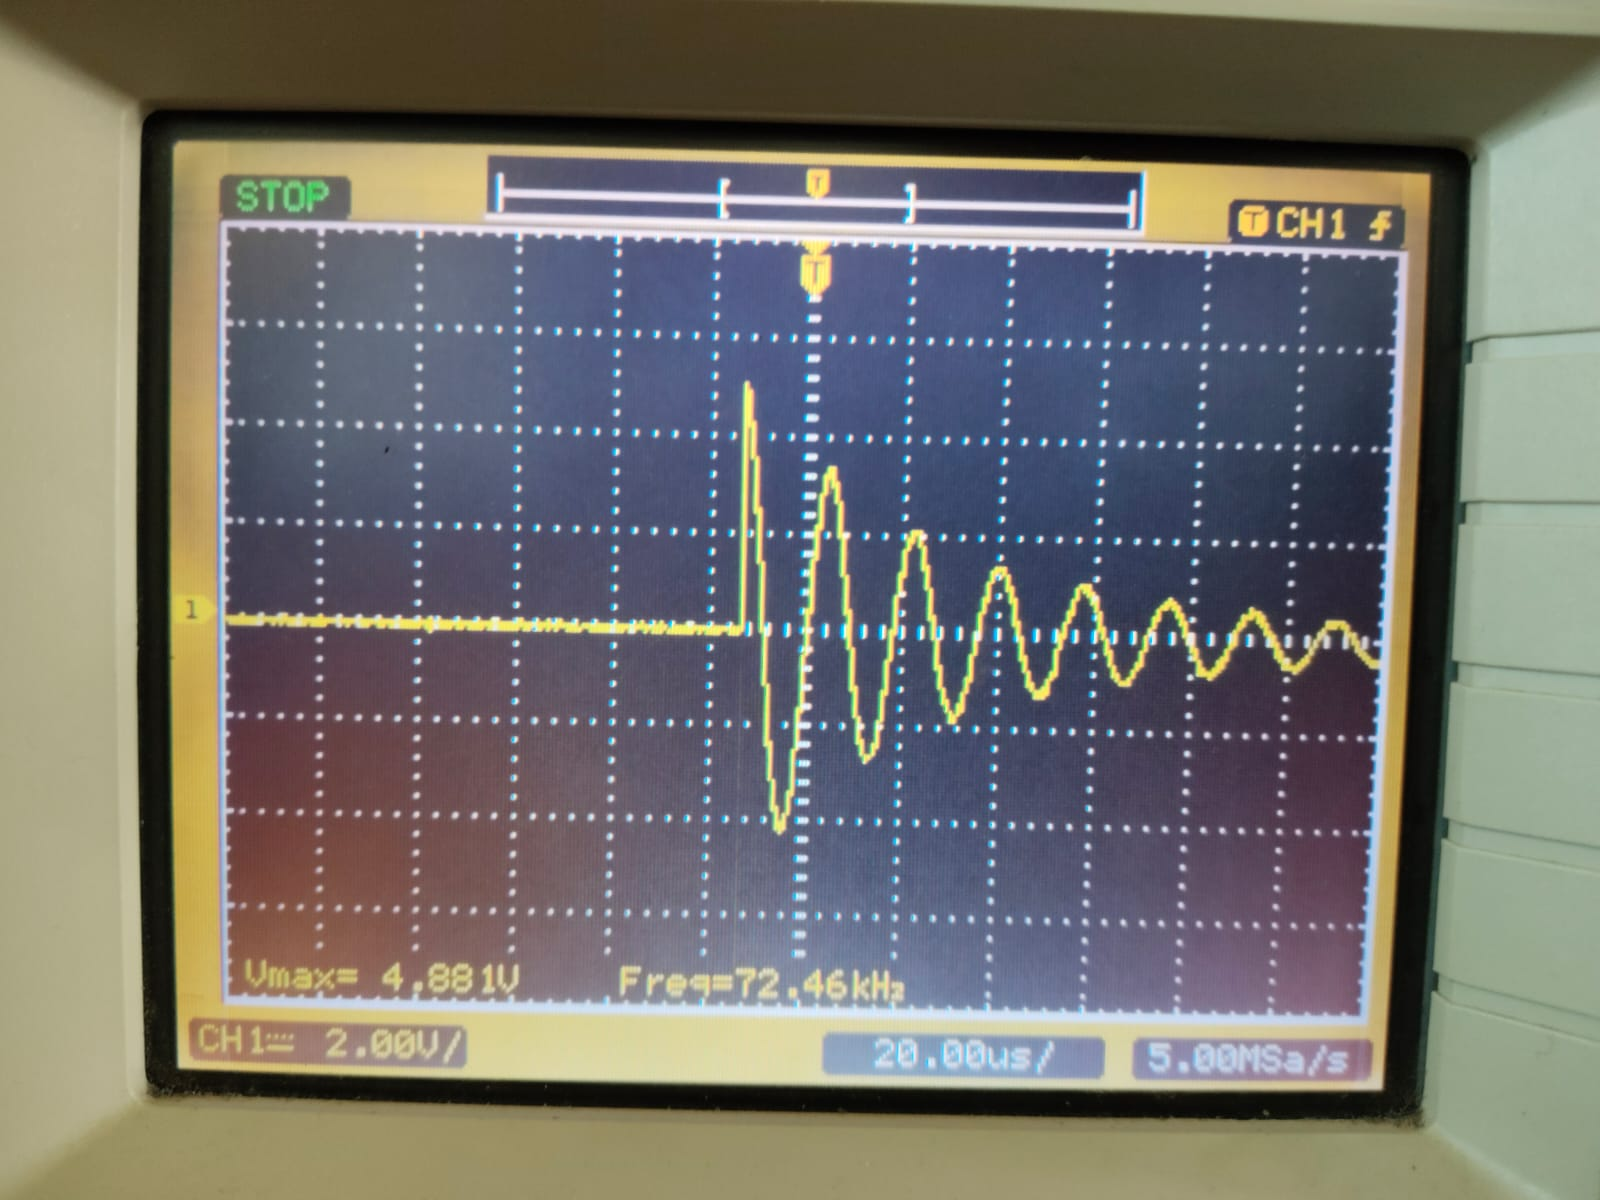
\includegraphics[width=0.7\textwidth]{figs/plot.jpeg}
    \caption{Transient Response of an LC Circuit}
\end{figure}

\subsection{Experimental Data and Observations}
\begin{itemize}
    \item Measured damped frequency: \SI{72.46}{\kilo\hertz}
    \item Theoretical natural frequency: \SI{156.05}{\kilo\hertz}
    \item Calculated damping ratio: \(\xi = 0.8855\)
    \item Estimated resistance: \SI{3.83}{\kilo\ohm} (possibly due to additional resistances)
\end{itemize}

\section{Effect of Resistance on Oscillations}

In an ideal LC circuit, where the inductor and capacitor have no resistance, energy oscillates continuously between the capacitor's electric field and the inductor's magnetic field. This results in a purely sinusoidal response at the natural frequency \(\Omega_n\):

\[
V(t) = V_0 \cos(\Omega_n t + \phi)
\]

However, real inductors and capacitors have internal resistance, which causes energy loss. The presence of resistance leads to damping, resulting in an exponentially decaying oscillation:

\[
V(t) = V_0 e^{-\alpha t} \cos(\Omega_d t + \phi)
\]

where \(\alpha = \xi \Omega_n\) is the decay rate.

\subsection{Illustrative Diagrams}

\begin{figure}[H]
    \centering
    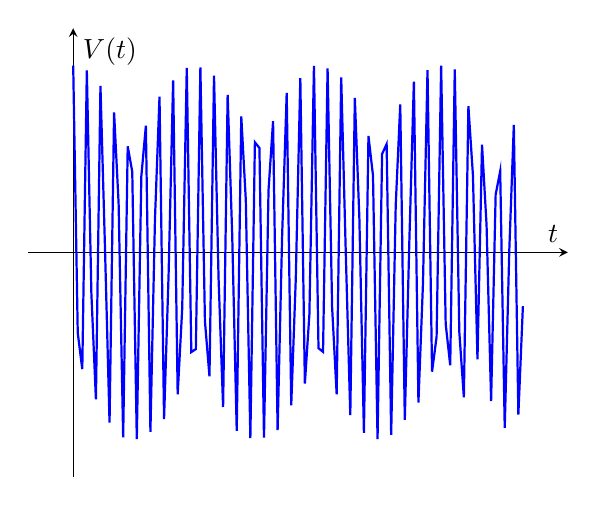
\begin{tikzpicture}
        \begin{axis}[
            domain=0:6.5,
            samples=100,
            axis x line=middle,
            axis y line=middle,
            xlabel={$t$},
            ylabel={$V(t)$},
            xtick=\empty,
            ytick=\empty,
            enlargelimits=true,
            clip=false
        ]
        \addplot[blue, thick] {cos(deg(deg(x*180/3.14)))};
        \end{axis}
    \end{tikzpicture}
    \caption{Ideal LC circuit response: Continuous sinusoidal oscillation}
\end{figure}


\begin{figure}[H]
    \centering
    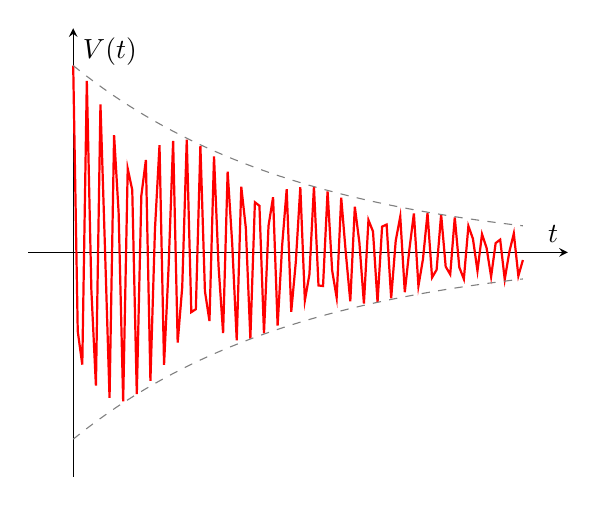
\begin{tikzpicture}
        \begin{axis}[
            domain=0:6.5,
            samples=100,
            axis x line=middle,
            axis y line=middle,
            xlabel={$t$},
            ylabel={$V(t)$},
            xtick=\empty,
            ytick=\empty,
            enlargelimits=true,
            clip=false
        ]
        \addplot[red, thick] {exp(-0.3*x) * cos(deg(deg(x*180/3.14)))};
        \addplot[dashed, gray] {exp(-0.3*x)};
        \addplot[dashed, gray] {-exp(-0.3*x)};
        \end{axis}
    \end{tikzpicture}
    \caption{Damped LC circuit response: Exponentially decaying oscillation due to resistance}
\end{figure}


In the case of strong damping (\(\xi > 1\)), oscillations may not occur at all, leading to an overdamped response where the system slowly returns to equilibrium. If \(\xi = 1\), the system is critically damped and returns to equilibrium in the shortest possible time without oscillating.
\subsection{Decay Rate}
The decay rate (attenuation coefficient) \(\alpha\) determines how quickly oscillations decrease in amplitude due to resistance.\\
It is also related to the damping ratio as:
\begin{equation*}
    \alpha = \xi \Omega_n
\end{equation*}
\begin{equation*}
    \alpha = 0.8855 \times 980.39 \times 1000 = 868.135345 \times 10^3
\end{equation*}
The relation between decay rate and natural and damped frequency is given by:
\begin{equation*}
    \alpha = \sqrt{\omega_n^2 - \omega_d^2}
\end{equation*}
\begin{equation*}
    \alpha = \sqrt{\left(980.39 \times 10^3\right)^2 - \left(455.28 \times 10^3\right)^2}
\end{equation*}
\begin{equation*}
    \alpha = 868.27 \times 10^3
\end{equation*}
The above experimentally calculated decay rate matches closely with the theoretical value.\\ 

The amplitude of the oscillations follows an exponential decay:
\begin{equation*}
    V(t) = V_0 e^{-\alpha t} \cos(\Omega_d t + \phi)
\end{equation*}
where \(V_0\) is the initial amplitude.

The decay rate can also be experimentally determined using the logarithmic decrement method:
\begin{equation*}
    \delta = \ln \left(\frac{V_n}{V_{n+1}}\right)
\end{equation*}
where \(V_n\) and \(V_{n+1}\) are successive peak voltages. The decay rate is then:
\begin{equation*}
    \alpha = \frac{\delta}{T_d}
\end{equation*}
where \(T_d\) is the damped oscillation period.
\section{Analysis and Discussion}
\begin{itemize}
    \item The measured damped frequency is significantly lower than the ideal natural frequency, indicating non-negligible resistance in the circuit.
    \item The calculated resistance of \SI{3.83}{\kilo\ohm} seems too high for a typical inductor, suggesting additional resistive losses or measurement artifacts.
    \item Possible sources of extra resistance include inductor DC resistance, capacitor ESR, wiring resistance, and core losses.
\end{itemize}

\section{Conclusion}
The experiment demonstrated transient oscillations in an LC circuit and allowed for a comparison of theoretical and experimental results. The presence of resistance led to damping, reducing the oscillation frequency. Further investigation is needed to accurately determine the resistance components.

\section{Further Exploration}
\begin{itemize}
    \item Measure the inductor's DC resistance using a multimeter.
    \item Use a function generator to study forced oscillations.
    \item Experiment with different capacitor and inductor values to observe their effects n damping and frequency.
\end{itemize}

\section{Safety Precautions}
\begin{itemize}
    \item Handle charged capacitors carefully to avoid accidental discharges.
    \item Use components within their rated values to prevent damage.
    \item Ensure proper oscilloscope grounding to avoid erroneous readings.
\end{itemize}

\end{document}
